\documentclass{article}
\usepackage[utf8]{inputenc}
\usepackage{graphicx}

\title{Question 3}
\author{Jillian Henkel}
\date{May 2022}

\begin{document}

\maketitle

\section*{Introduction}
\section*{Question 1}
\subsection*{Methods}
\begin{figure}
    \includegraphics[scale=0.6]{iteration_bw.png}
    \caption{The black and white output for question 1.}
    \label{fig:iteration_bw}
\end{figure}

To determine the set of complex values that do not result in $z_{i + 1} = z_i + c$ diverging to infinity for a given initial condition: $z_0 = 0$, I generated a grid of points in the complex plane with boundaries $|x|, |y| \leq 2$. I created a Python function named "iteration()," which determines whether a given value of $c$ will result in values produced by the function leaving the given boundaries. I set the maximum number of iterations to 100, and for each point  $c$ in the grid, checked whether $|\mathfrak{R}(z_i)| > 2$ or $|\mathfrak{I}(z_i)| > 2$ at the ith iteration. If this is the case, the current value will be returned, and if it is not, it is concluded that the point remains bounded, and -1 is returned.
\subsection*{Results}
The first graph was produced by plotting the points that diverge in white and the points that remain bounded as black. To plot the second graph, plt.colorbar() was used. Both plots are examples of the mandelbrot set,  which is to be expected from this type of problem. At the edges of the set, we can see that small changes in $c$ can result in changes in the map's stability.


\section*{Question 2}
\subsection*{Methods}
In this question, I reproduced the results found in the provided paper. This was achieved by using Lornez's equations: 
\begin{eqnarray}
\dot X &=& -\sigma(X-Y)\\ \nonumber
\dot Y &=& rX -Y - XZ\\ \nonumber
\dot Z &=& -bZ + XY \nonumber
\end{eqnarray}
These equations were implemented in the Python function and ode solver was used to numerically integrate the equations from t=0 to t=60, with initial condition $W_0 = [X_0, Y_0, Z_0] = [0, 1, 0]$, and $\sigma = 10$, $r = 28$ and $b = 8/3$. The time evolution of Y over the first 3000 iterations of Lornez's equations were plotted, resulting in the reproduction of figure 1 in his paper. Doing the same for iterations 1400 to 1900 reproduced figure 2 of the paper. Lastly, I repeated the numerical integration done initially with the starting conditions $W_0' = W_0 + [0, 10^{-8}, 0]$.

\subsection*{Results}
The graphs produced match the graphs found in Lornez's paper. The graphs suggest that predicting the long-time behavior of weather will be difficult.
\begin{figure}
    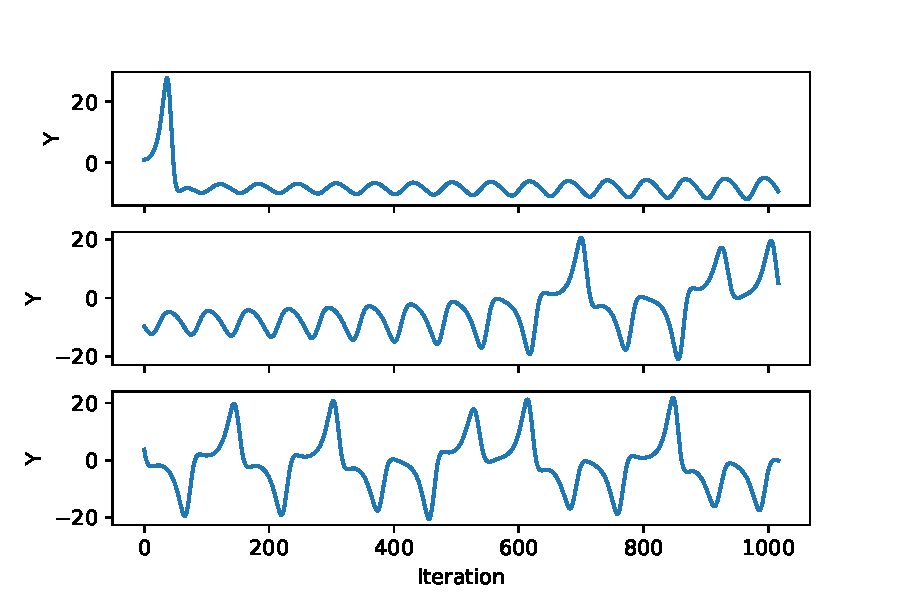
\includegraphics[scale=0.6]{Figure1.pdf}
    \caption{The recreation of Figure one in Lornez's paper.}
    \label{fig: Figure 1}
\end{figure}

\end{document}


